\documentclass{standalone}
\usepackage{tikz}
\begin{document}

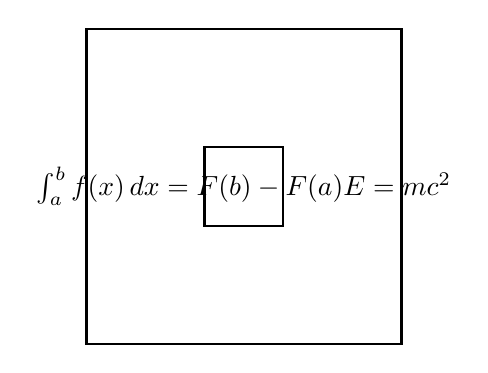
\begin{tikzpicture}[scale=1]
    % Draw the outer white square with a black border
    \draw[black, thick] (0, 0) rectangle (4, 4);

    % Fill the inner white square with white color
    \fill[white] (1, 1) rectangle (3, 3);

    % Draw the inner black box inside the white square
    \draw[black, thick] (1.5, 1.5) rectangle (2.5, 2.5);

    % Add some mathematical symbols and equations inside the inner black box
    \node at (2, 2) {
        $\int_{a}^{b} f(x) \, dx = F(b) - F(a)$ \\
        $E = mc^2$
    };
\end{tikzpicture}

\end{document}